\section{Die Bilderkennung}

Das Ziel der Bilderkennung ist es, zwei Punkte zu identifizieren, von denen man den Abstand in den Weltkoordinaten kennt. Anschließend kann man dann durch eine Koordinatentransformation von den Bildkoordinaten zu den Weltkoordinaten die Position der Kamera in der Welt in Relation zum bekannten Objekt bestimmen. Für dieses Objekt haben wir ein rotes Rechteck gewählt.

\subsection{Bildvorverarbeitung}

Zuerst soll das Bild so angepasst werden, dass das rote Rechteck einfacher identifizierbar wird. 
Normalerweise würde man damit beginnen, das Bild erstmal vorzuglätten (zum Beispiel mit einem Gauss-Filter) um Rauschen zu minimieren. Dies hat sich aber aus Performancegründen als nicht so hilfreich herausgestellt. Stattdessen kann hier gut die Eigenschaft, dass das Rechteck rot ist, verwendet werden. Wenn man sich die RGB-Kanäle (a, b und c) anschaut, fällt auf, dass das rote Rechteck sehr hell im roten Kanal ist, allerdings fast gar nicht in dem blauen und grünen Kanal sichtbar ist. Alle anderen Farben haben auch einen Blau- oder Grünanteil. Aus diesem Grund wird im ersten Schritt ein Graustufenbild (e) erzeugt, in dem der blaue und grüne Kanal vom roten Kanal abgezogen werden.

\begin{center}
\begin{table}[ht]
\begin{tabular}{c c c}
\begin{subfigure}{0.3\textwidth}\centering

\includegraphics[scale=0.08]{Figures/rotkanal.png} \vspace{-3.5mm}\caption{Rotkanal}
\end{subfigure}&
\begin{subfigure}{0.3\textwidth}\centering

\includegraphics[scale=0.08]{Figures/gruenkanal.png} \vspace{-3.5mm}\caption{Grünkanal}
\end{subfigure}&\begin{subfigure}{0.3\textwidth}\centering

\includegraphics[scale=0.08]{Figures/blaukanal.png} \vspace{-3.5mm}\caption{Blaukanal}
\end{subfigure}\\ 
\begin{subfigure}{0.3\textwidth}\centering

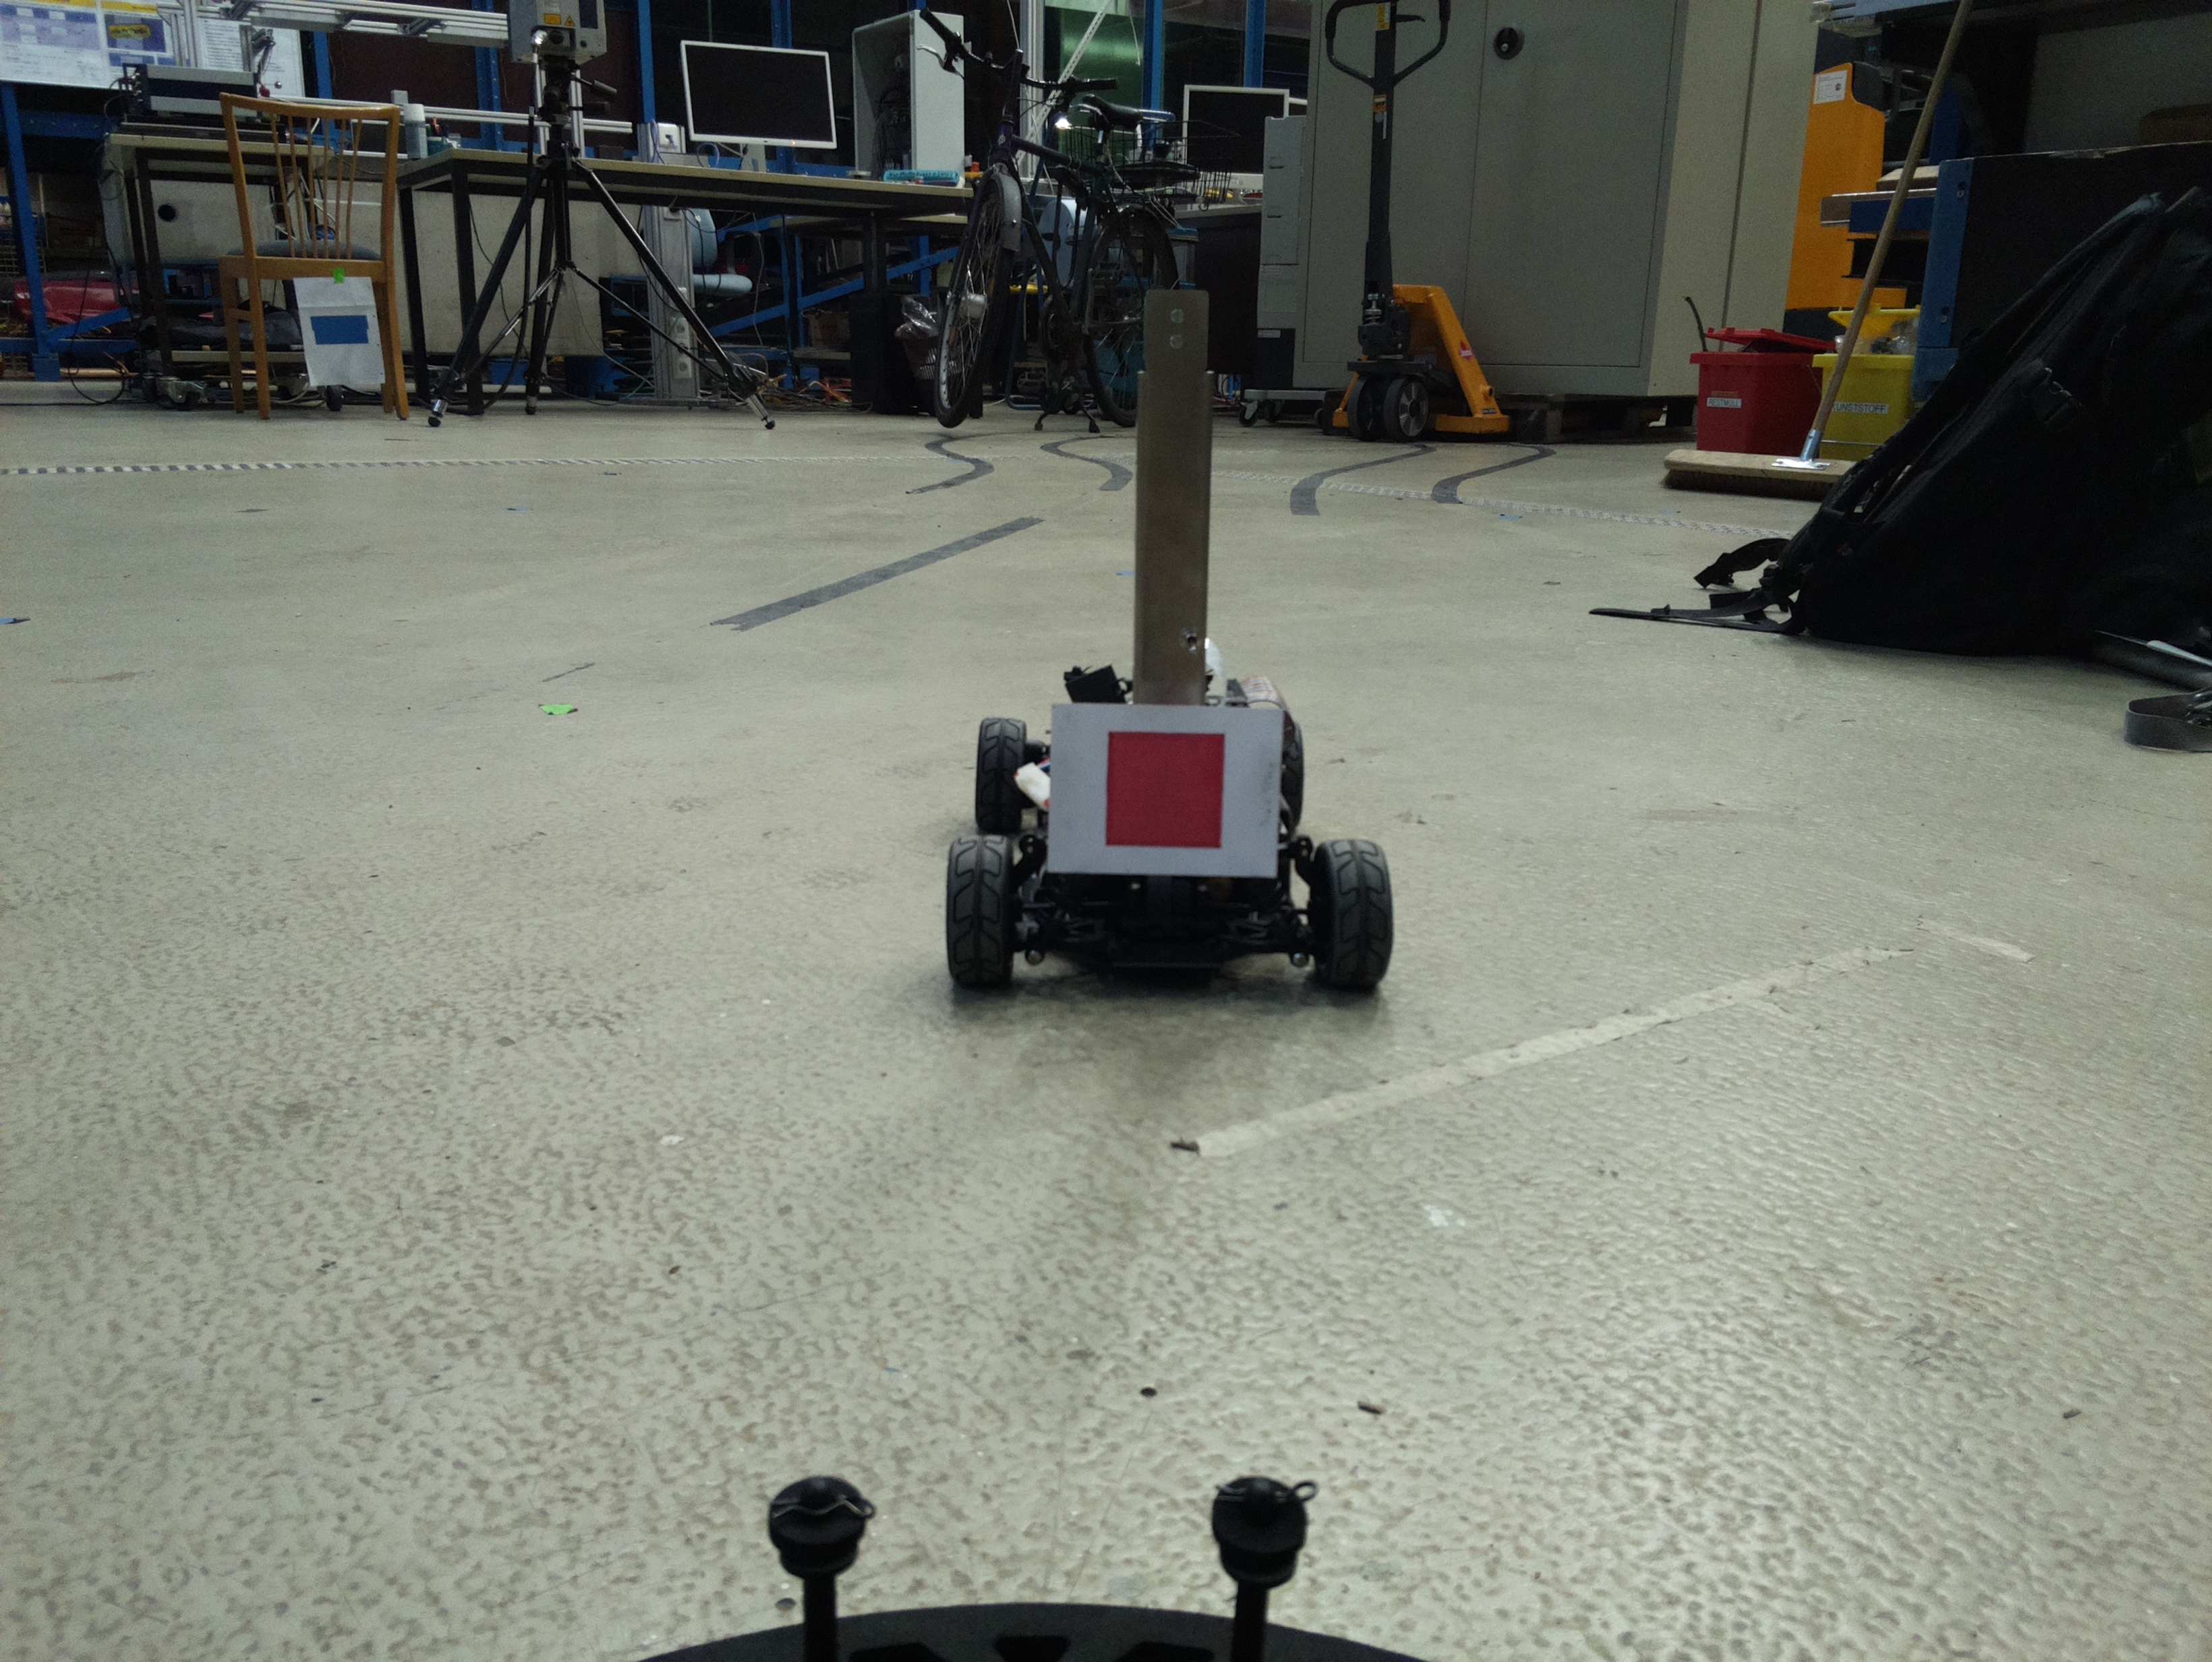
\includegraphics[scale=0.08]{Figures/rechteckbild.png} \vspace{-3.5mm}\caption{Farbbild}
\end{subfigure}&\begin{subfigure}{0.3\textwidth}\centering

\includegraphics[scale=0.08]{Figures/r-g-b.png}  
\vspace{-3.5mm}\caption{Rot-0.5(Grün+Blau)}
\end{subfigure}&\begin{subfigure}{0.3\textwidth}\centering

\includegraphics[scale=0.08]{Figures/binaerbild.png} \vspace{-3.5mm}\caption{Binärbild}
\end{subfigure}
\end{tabular}
\end{table}
\end{center}
\vspace{-5mm}

In diesem Graustufenbild (e) sind nun hauptsächlich helle Rottöne sichtbar. Nun kann ein Binärbild (f) erstellt werden, indem alle Grautöne über einem Schwellenwert weiß dargestellt werden und alle anderen schwarz. 


\subsection{Rechteckserkennung}

Nun sollen die Eckpunkte des Rechteckes gefunden werden. Im ersten Schritt wird ein Gitter über das Bild gelegt, das so fein gewählt wird, dass ein Gitterpunkt auf jeden Fall im Rechteck liegen muss. Dafür wird angenommen, dass das Rechteck eine Mindestgröße im Bild hat und nicht zu weit weg ist. Ob ein Gitterpunkt $(x_1,y_1)$ nun wahrscheinlich in einem Rechteck liegt, wird mithilfe des Algorithmus 1 festgestellt.\\


\begin{figure*}[h]
  \centering
\begin{minipage}[t]{0.5\textwidth}
\centering
\vspace{-0.4cm}
\renewcommand\figurename{Algorithm}
\begin{algorithm}[H]
\caption{Pseudo-Code}\label{euclid}
\begin{algorithmic}[1]
\State $(x,y) = (x_1, y_1)$
\While {$I(x,y) = $ white}
	\State $ y = y - 1$
\EndWhile

\State $ y_2 = y$
\State $(x,y) = (x_1, y_1)$
\While {$I(x,y) = $ white}
	\State $ y = y + 1$
\EndWhile
\State $y_3 = y$
\end{algorithmic}
\end{algorithm}

\end{minipage}\hfill
  \begin{minipage}[t]{0.35\textwidth}
    \centering
    \raisebox{-\height}{\includegraphics[width=1\textwidth]{Figures/rechteckgrafik.pdf}}
    \vspace{-0.2cm}
    \caption{Beispiel-Rechteck}\label{fig:xx}
  \end{minipage}\hfill

\end{figure*}
%
Dies bestimmt den Punkt $(x_1,y_2)$ und $(x_1,y_3)$. 
Anschließend lässt sich der Mittelpunkt {$(x_1,y_m)=(x_1,\frac{y_2+y_3}{2})$ bestimmen. Nun wird der gleiche Algorithmus nochmal in x-Richtung durchgeführt mit Startwert $(x_1,y_m)$ um $x_l$ und $x_r$ zu finden. Um leicht schräge Seiten auszugleichen, wird nun der Algorithmus auf $(x_l+a,y_m)$ und $(x_r-a,y_m)$ angewandt, um die die vier Rechtecksecken $(x_{ol},y_{ol}),(x_{or},y_{or}),(x_{ul},y_{ul})$ und $(x_{ur},y_{ur}))$ zu finden.\\
%
Nun wird noch überprüft, ob die gefundenen Ecken ein sinnvolles Rechteck bilden. Dafür darf $y_{ol}-y_{ul}$ nicht mehr als $ 30\% $ größer oder kleiner als $y_{or}-y_{ur}$ oder $x_r-x_l$ sein, da das Rechteck leicht nach hinten gekippt sein kann (vorausfahrendes Auto lenkt). Außerdem soll noch $\frac{y_m-y_{ol}}{y_m-y_{or}}$ ungefähr $\frac{y_{ul}-y_{m}}{y_{ur}-y_{m}}$ sein. Wenn diese Bedingungen eingehalten werden, handelt es sich wahrscheinlich um ein Rechteck.\\
%
Um möglichst schnell den richtigen Startpunkt $(x_1,y_1)$ zu finden, wird spiralförmig um den Mittelpunkt des im letzten Bild gefundenen Rechtecks gesucht.
